\section{Infraestrutura Tecnológica do RIL}\label{sec:inf-tecnologias}

    Nesta secção, vamos explorar a infraestrutura tecnológica essencial para o projeto, abrangendo a plataforma OutSystems, ferramentas de integração, nuvens e outros componentes vitais.

        \subsection{Integração com Ferramentas na Nuvem}\label{secsec:azure-integracao}
        
        No projeto temos uma forte integração com uma panóplia de ferramentas presentes na nuvem com uma forte e complexa rede de APIs que interligam os diferentes sistemas entre si de forma segura e eficaz. 
        
        \subsubsection{Azure}\label{secsec:azure}

        O Azure desempenha um papel fundamental no projeto e muitas funcionalidades desta nuvem são extensamente utilizadas, como por exemplo:
        
        \begin{itemize}
            \item \textbf{Azure AD}(Active Directory)\textbf{:} Usado para autenticação dos utilizadores;
            \item \textbf{Máquinas Virtuais}(VMs)\textbf{:} Várias máquinas virtuais são usadas por várias razões.
            
            Temos duas regiões ativas para as VMs, UK South e UK West, para um determinado utilizador é selecionado aquele servidor relativamente ao qual o utilizador apresenta menor latência. Este procedimento serve como uma camada de segurança contra desastres naturais ou humanos caso um dos \textit{datacenters} seja comprometido.
            
            Existem dois ambientes principais no Azure do projeto, \textit{RIL} e \textit{RIL SandPit}, onde o primeiro contém todas as VMs relacionadas com o ambiente de produção e o segundo todas as relacionadas com os outros ambientes e as suas diferentes finalidades. Cada ambiente tem a sua própria máquina virtual atribuída, no entanto os conceitos de \textit{scale up} e \textit{scale out} são relevantes na sua organização;

            \textbf{Scale Up:} Refere-se ao aumento da capacidade de um sistema ou máquina virtual aumentar os recursos de um ou mais nodos já existentes da rede, ou neste caso, de uma só VM. Isto pode envolver o aumento do poder computacional da máquina como aumentar a quantidade de CPU, memória RAM ou armazenamento. Geralmente, este método é usado quando é necessário fazer uma tarefa única que requer muitos recursos apenas da máquina que a vai realizar, como, por exemplo, um deploy bastante extenso;

            \textbf{Scale Out:} Diz respeito à expansão horizontal do sistema, cuja metodologia se foca na distribuição da carga entre vários nós ou servidores em vez de fortalecer um único dispositivo. É mais eficaz para lidar com cargas de trabalho dinâmicas, e é útil, por exemplo, nas horas de maior ou menor afluência de utilizadores\cite{scale-up-scale-out};

            \item \textbf{Azure Firewall:} Utilizado para o controlo de tráfego no ambiente Azure, gerir e garantir a segurança das comunicações;

            \item \textbf{Azure PagerDuty:} Para gerar alertas críticos e mais fácil e eficazmente responder a estes;
            
            \item \textbf{Azure Storage \& logs:} O armazenamento não alocado às VMs tem a função de guardar logs de todas as partes da aplicação. São utilizadas no projeto em conjunto com, por exemplo, as \textbf{Logic Apps} para criar e orquestrar fluxos de trabalho automatizados como, por exemplo, inspecionar as tabelas de SQL de OutSystems dentro das VMs com a componente de Azure de SQL e retirar os logs relevantes e armazená-los. Também servem para inspecionar os logs em si, e caso aconteça algo fora do normal, enviar um alerta P\textit{X}. São usadas também \textbf{Function Apps} desenvolvidas em .NET ou Python nos casos que pedem um pouco mais de controlo, como interações com os \textit{endpoints} do MongoDB.
            
            % \item \textbf{Availability Logs:} Os Availability Logs são parte integrante do monitoramento contínuo do projeto. O Azure realiza pings regulares aos deploys, gerando logs de disponibilidade que são cruciais para identificar e resolver problemas em tempo hábil.
        \end{itemize}
        
        \subsubsection{Atlas}\label{secsec:atlas}
        
            O Atlas é a nuvem de armazenamento do MongoDB, é usado no caso do projeto para armazenar todos os dados relacionados com a base de dados, desempenhando um papel central na gestão e teste destes. 

            Muitas vezes é necessário fazer \textit{datafixes}, uma alteração à base de dados para os dados ficarem como o cliente espera. Muitas vezes \textit{datafixes} são necessários devido a um problema no código que causou alguns dados da BD a serem guardados numa forma indevida, ou alguma ação que o utilizador fez que tenha que ser revertida. \textit{Datafixes} são também muitas vezes usados mesmo em ambientes de teste, facilitando o processo de reprodução de problemas.

            Para mais informação acerca do uso da plataforma, por favor consulte à secção \hyperref[sec:ferramentas-atlas]{Plataforma Atlas}.

        \subsubsection{Nuxeo}\label{secsec:nuxio}
        
            O Nuxeo é outra peça-chave no projeto, integrando-se com o \hyperref[secsec:apis]{Power Config API} é usado para armazenar os documentos carregados pelos utilizadores na aplicação.

            É importante que esteja bem integrado com Azure para impedir que os URLs dos documentos não estejam acessíveis a qualquer um, pelo que tem que ter um registo dos utilizadores e das permissões de cada um. Serve como uma base de dados para guardar os documentos sensíveis dos utilizadores como os contratos, documentos de mudanças de contratos, certificados, relatórios, etc. % \hyperref[secsec:apis]{APIs}. 
        
        \subsubsection{SendGrid}\label{secsec:sendgrid}

            Embora não faça parte da infraestrutura de nuvem que manipula informações sensíveis, \href{https://sendgrid.com/en-us/pricing}{SendGrid} é utilizado como uma solução externa para o envio de e-mails para os utilizadores. É um API que é usado exclusivamente pelo código em OutSystems.
    
        \subsection{APIs}\label{secsec:apis}

            Nesta secção vamos explorar como os APIs do projeto funcionam e estão expostos para que todas estas ferramentas distintas possam comunicar entre si com sucesso e de forma segura.

            No início do projeto, uma grande parte do código encontrava-se em APIs externos em código .NET e C\#, para, por exemplo, OutSystems ter acesso à base de dados de Mongo. No entanto com o tempo, a tendência foi converter estes blocos de código em lógica que pudesse correr mesmo dentro da OutSystems sob a forma de extensões ou módulos. No seu estado atual, o projeto tem os APIs internos de OutSystems e o API Org Config.

            \subsubsection{APIs OutSystems}\label{secsec:apis-os}
                Trata-se de APIs internos da OutSystems usados para comunicação entre módulos ou serviços do ecossistema de OutSystems como o Service Studio e o Service Center. 

                Dentro da próprio OutSystems também foram criados vários módulos \textit{\_Drv} que são a segunda camada mais baixa da organização no projeto, estes módulos utilizam uma extensão da OutSystems que se pode visualisar através do Service Center como demonstrado na Figura \ref{fig:os-extension}, foi criada com o propósito exclusivo de comunicar com a base de dados de MongoDB que é um exemplo de uma das formas como o projeto evoluiu para ser integrado de uma forma mais estreita com o ecossistema de OutSystems.

                \begin{figure}[htbp]
                    \centering
                    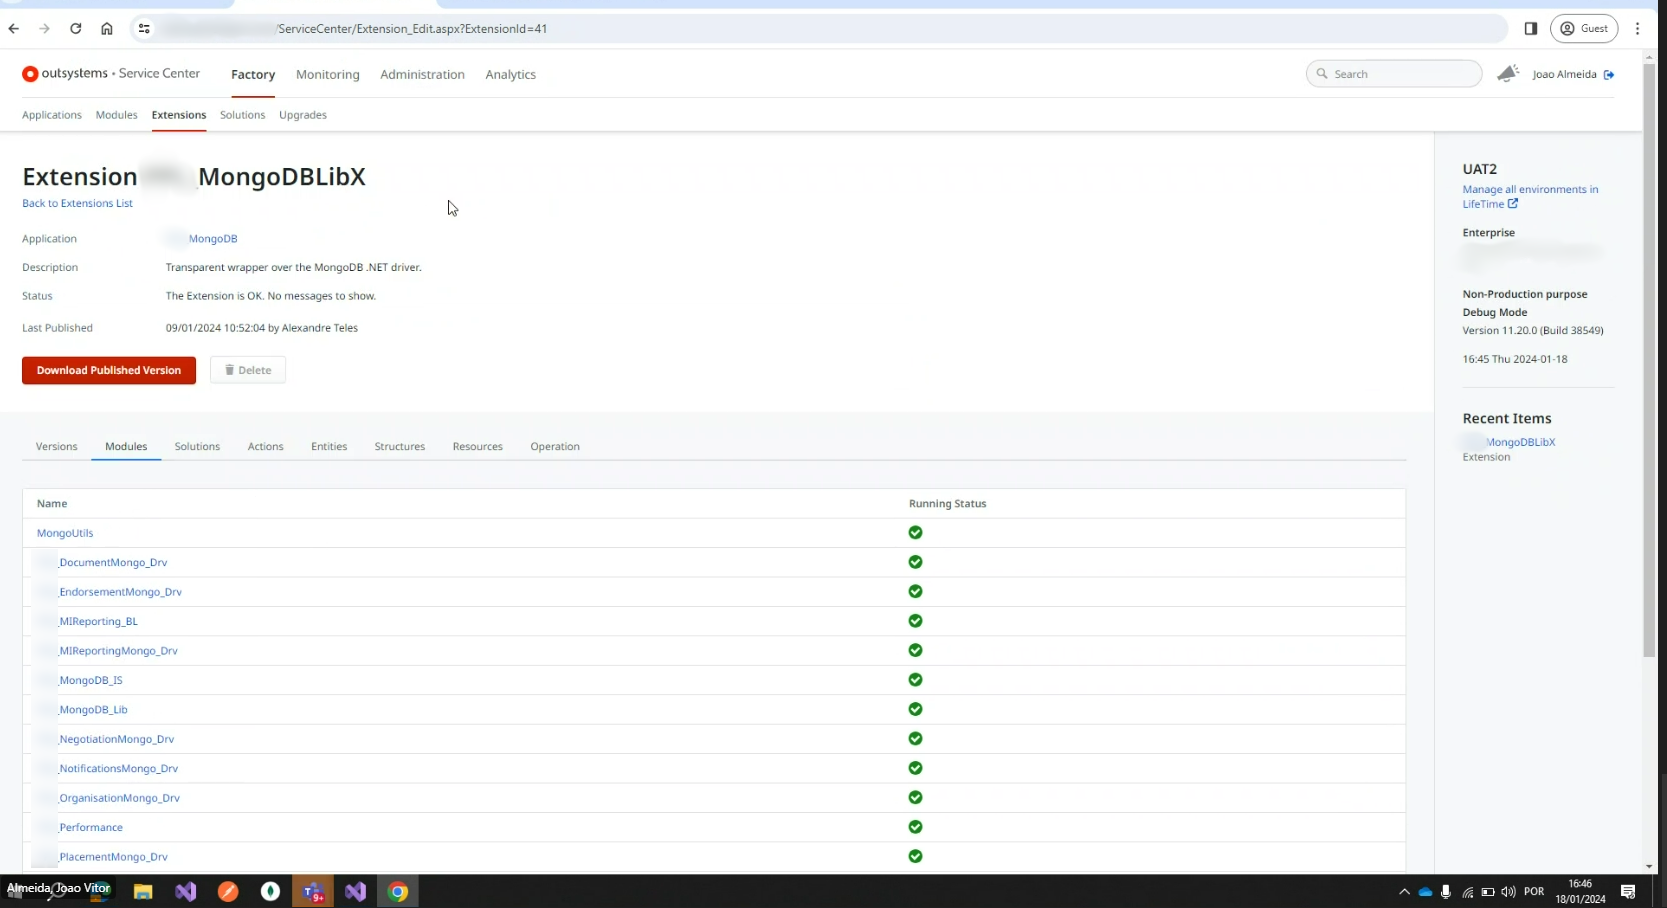
\includegraphics[scale=0.35]{imgs/ExtensionEndpoint-outsystems.png}
                    \caption{Extensão da OutSystems}\label{fig:os-extension}
                    \source{Documentação Interna}
                \end{figure}

            \subsubsection{API Org Config}\label{secsec:api-org-config}
            
                Desenvolvido em .NET fora de OutSystems, o papel do Org Config é ter um método de comunicar com mongoDB, Nuxeo, Azure e OutSystems de forma consistente, garantindo não haver dessincronização entre os dados.

                Por exemplo, o registo dos utilizadores que existem em cada ambiente e as suas permissões devem constar da base de dados MongoDB, o principal sítio que mantém os dados dos utilizadores, no Nuxeo, para que um documento de um cliente possa ser acedido apenas por esse cliente e o URL não seja público. \\
                Estão guardados também no Azure, para efeitos de análise de dados e erros.

                Desta forma o processo é simplificado, exportando a lógica de sincronização entre vários serviços para o API Org Config, que disponibiliza a lógica em mais de uma dúzia de funções visiveis na Figura \ref{fig:api-org-config}.

            \begin{figure}[htbp]
                \centering
                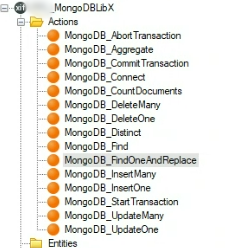
\includegraphics[scale=0.80]{imgs/API-Org-Config.png}
                \caption{Usable actions by the API}\label{fig:api-org-config}
                \source{Documentação Interna}
            \end{figure}
        
        \subsection{Versionamento}\label{secsec:versionamento}

            Como alternativa à utilização de uma ferramenta direta de controlo de versionamento, foi elaborado um sistema de vários ambientes, cada um com uma função específica, por onde o código viaja antes de finalmente se encontrar no ambiente final de produção usado pelos utilizadores.
        
            Os números das versões regem-se por majors, minors e hotfixes.

            \[
                \text{Version: }
                  \underbrace{2\vphantom{(y)}}_\text{major} \text{.}
                  \underbrace{3\vphantom{(y)}}_\text{minor} \text{.}
                  \underbrace{5\vphantom{(y)}}_\text{hotfix} \text{.}
              \]

            \begin{itemize}
                \item \textbf{Major:} A versão principal que indica grandes atualizações ou alterações no software. Aumentar o número da versão principal implica mudanças significativas como, por exemplo, uma reestruturação da plataforma e pode resultar em incompatibilidades com versões anteriores;

                \item \textbf{Minor:} Reflete atualizações menores, melhorias ou adições em partes focadas da aplicação, como, por exemplo, alteração do fluxo para criar um contrato;

                \item \textbf{Hotfix:} Uma correção rápida para resolver problemas críticos, bugs ou \textit{defects}. A diferença entre hotfixes não costuma ser significativa, pelo que não é geralmente referida. Quando se menciona a versão da plataforma, geralmente inclui-se apenas da major e da minor, por exemplo: Versão 2.3.
                
            \end{itemize}
            
            \subsubsection{Ambientes}\label{secsec:ambientes}

                Nesta seção, apresenta-se uma visão abrangente dos ambientes envolvidos no processo de desenvolvimento, teste e implementação.

                É crucial compreender o propósito de cada ambiente para garantir uma implementação eficaz da metodologia AD Factory. A Tabela \ref{table:desc-ambinetes} oferece uma descrição detalhada dos diferentes ambientes, destacando a sua utilização principal e os principais utilizadores envolvidos.

                \textbf{AD Factory}: A AD Factory (Application Development Factory) representa uma abordagem organizada no projeto, focada na estruturação eficiente do ciclo de desenvolvimento. Divide-se em várias linhas de trabalho (PODs) que se refletem em várias equipas, a AD Factory coordena desde a fase de design até aos testes num processo estruturado. Durante a fase de design, as decisões detalhadas são tomadas em cada POD, com histórias de utilizadores aprovadas por um Analista de Dados de Negócios (BDA). A fase de construção e testes seguem-se conforme planos elaborados em sessões de \textit{sprint}, utilizando quadros JIRA específicos para cada POD. Acompanha-se o progresso através do JIRA, com relatórios, fluxos principais e a lista de \textit{defects} bem categorizados.

                \begin{table}[htbp]
                    \centering
                    \begin{tblr}{
                    colspec={|X|X[3]|X[1]|}, row{1} = {c}, hlines={lightgray}, vlines={lightgray},
                    }
                    \textbf{Ambiente} & \textbf{Descrição / Uso} & \textbf{Principais Utilizadores} \\
                    %DEV
                    Desenvolvimento (DES) & Ambiente de desenvolvimento para desenvolver as ``User Stories''. & Programadores \\
                    %STG
                    Teste (TES1) & Utilizado para teste de sistema com DES, integração e regressão. & Programadores e Tests na sprint \\
                    %DAD
                    Desenvolvimento para AD Factory (DED) & Ambiente para apoiar o desenvolvimento do ramo de código AD Factory em paralelo com as correções e correções de bugs no ramo DES. & Programadores da AD Factory \\
                    %SAD
                    Teste para AD Factory (TES2) & Ambiente temporário para apoiar os testes do ramo DED. & Programadores da AD Factory e Testes na sprint \\
                    %E2E
                    Ponta a Ponta (P2P) & Utilizado para testes ponta a ponta de temas discutidos nas \textit{sprints}. & Equipa de Testes E2E \\
                    %UAT
                    Aceitação do Utilizador (ADU) & Utilizado para testes de aceitação do utilizador. Teste de upload de configuração da organização e verificação de processos com empresas. & Equipa de Testes da RIL \\
                    %PERF
                    Performance (PCE) & Utilizado para testes de desempenho. & Equipa de Testes de Performance \\
                    %PRE
                    Pré-Produção (PREP) & Ambiente para auxiliar o ambiente PRO, para testes, configuração, testes de mercado e integração de APIs. & Equipa de Testes de Mercado da RIL \\
                    %JIT
                    Teste Integração Conjunta (TIC) & Utilizado para integração do mercado com a API exposta externamente. & Devs e entidades externas \\
                    %DEMO
                    Demonstração (SHOW) & Ambiente com cópia de PRO para efeitos de demonstração. & Gestão de Relações RIL \\
                    %SUP
                    Produção de Suporte (AUX) & Ambiente publicado com uma versão do código de produção quase idêntico, permitindo solucionar problemas sem impactar o ambiente de produção. & Equipa de Execução \\
                    %PRDO
                    Produção (PRO) & Ambiente de produção disponível aos clientes. Testes de Aceitação Operacional. Teste de Penetração da RIL. & Clientes da RIL, administradores da RIL e Equipa de Execução \\
                    \end{tblr}
                    \caption{ Descrição dos ambientes }\label{table:desc-ambinetes}
                    \source{Documentação Interna}
                \end{table}

            \subsubsection{Deployment Agreggator}\label{secsec:deployment-agreggator}

            \begin{figure}[htbp]
                \centering
                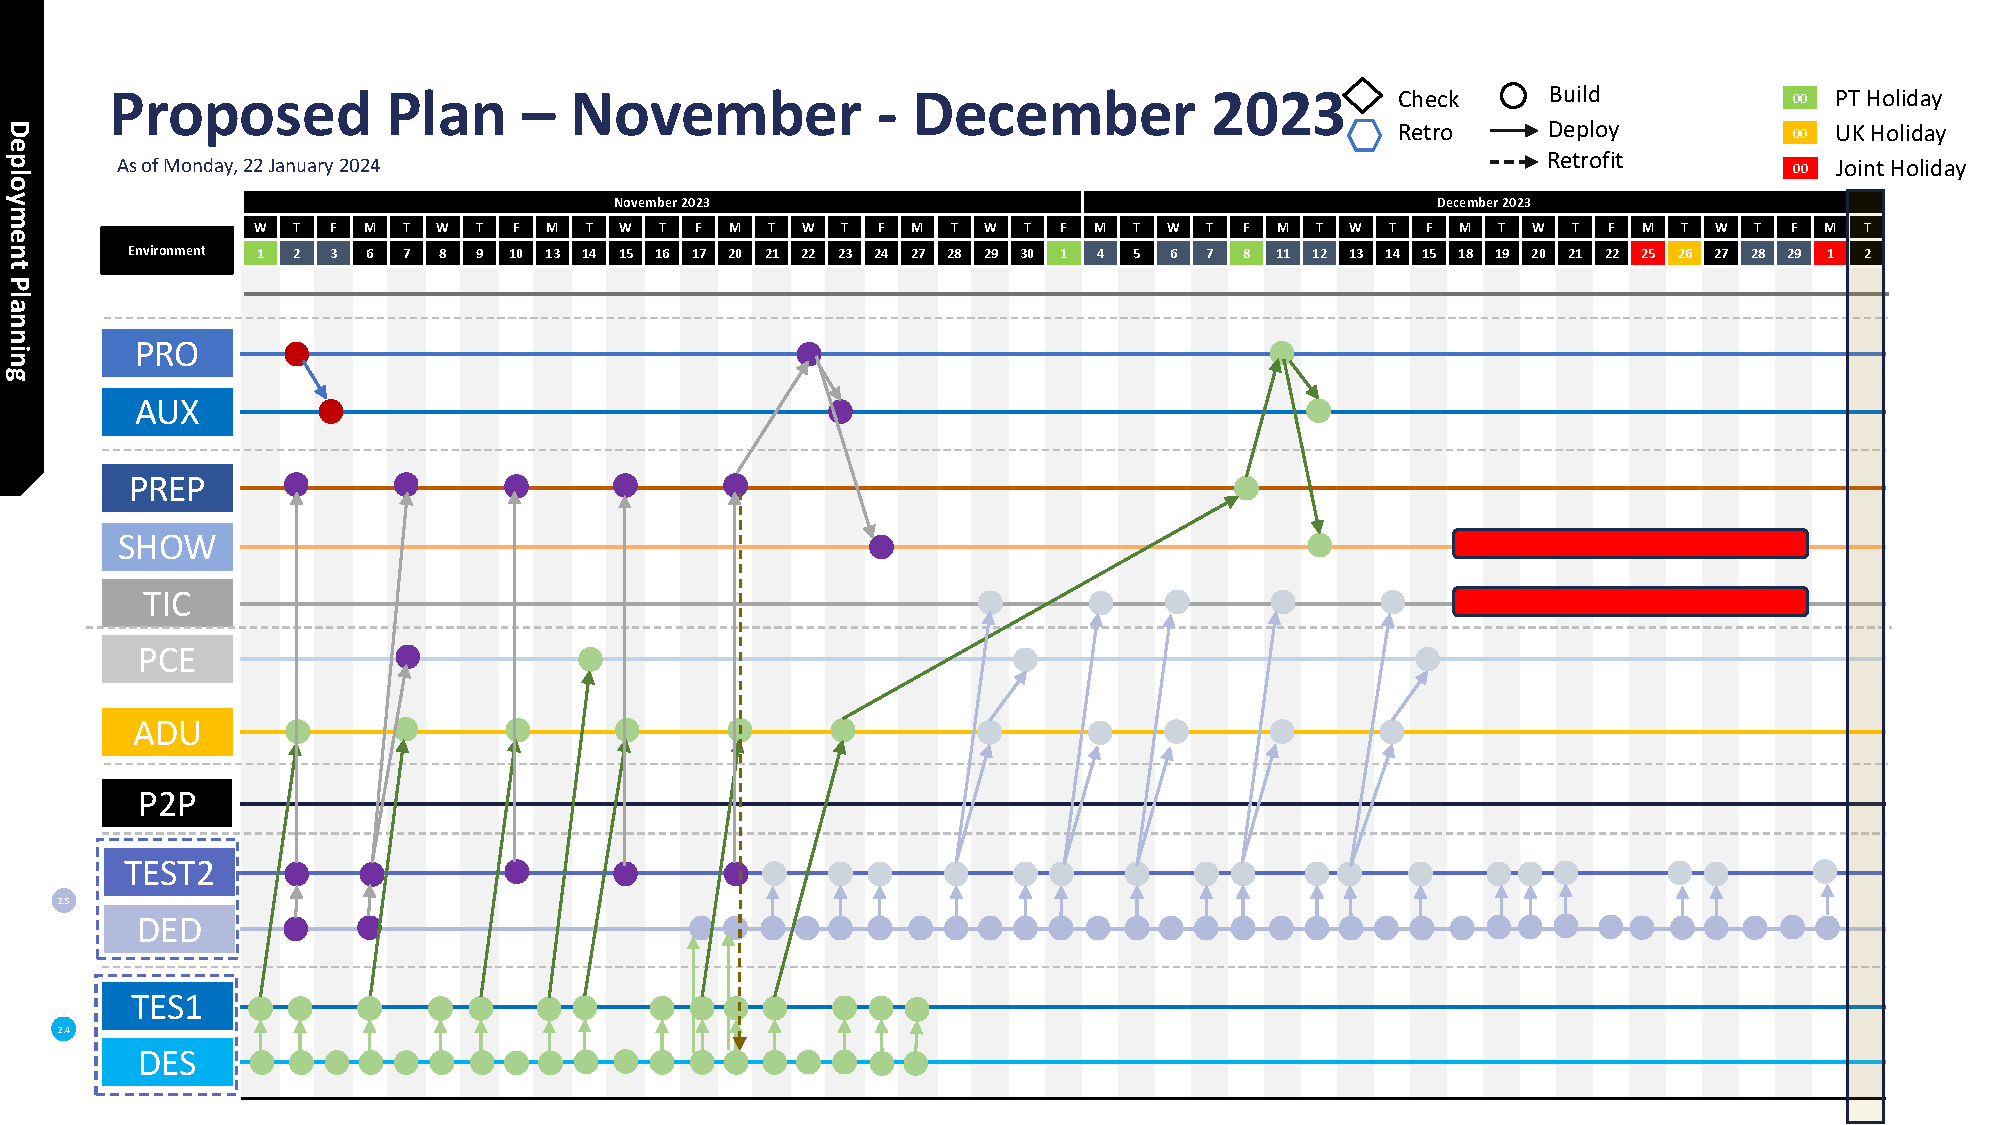
\includegraphics[width=\textwidth]{imgs/DeploymentAggregator-Example.pdf} % You can replace 'example-image-a' with the path to your actual image
                \caption{Deployment Aggregator}\label{fig:deployment-aggregator}
                \source{Protótipo de um Deployment Aggregator com base na Documentação Interna}
            \end{figure}

            A cada par de meses, é gerado um novo ``Deployment Aggreggator'', um cronodiagrama que detalha o fluxo do código entre ambientes e as datas em que estes deploys devem ocorrer.
             
            Pode ter também a representação de férias ou freezes, um paradigma bastante usado em empresas, que se refere a períodos em que não há deploys e a maior parte dos trabalhadores não estão de serviço, por exemplo, por estarem de férias, podendo, no entanto, haver deploys de emergência. Este período é representado por retângulos vermelhos no deployment agreggator, Figura \ref{fig:deployment-aggregator}.
            
            Existem dois ambientes de desenvolvimento, neste exemplo, TEST1 e TEST2, ambos com um ambiente de testes, DES e DED, respetivamente. Foram criados os dois para possibilitar o trabalho em duas \textit{sprints} de desenvolvimento, duas minors diferentes, por exemplo, simultaneamente. No protótipo de exemplo dado, está-se a trabalhar na minor 2.4 no ambiente DES e na minor 2.5 no ambiente DED. É possível ver que o código da 2.4 vai chegar a produção no dia 11 de dezembro, e que o código com a 2.5, que irá ser fundido no ambiente ADU, não tem ainda uma data definida para a chegada à produção devido ao freeze.

            % todo: o que é um retrofit tmb